\documentclass[compsoc, 10, draftclsnofoot, onecolumn]{IEEEtran}
\usepackage{listings}
\usepackage{underscore}
\usepackage[bookmarks=true]{hyperref}
\usepackage[utf8]{inputenc}
\usepackage[english]{babel}
\usepackage{placeins}
\usepackage{indentfirst}
\usepackage{graphicx}
\usepackage{hyperref}
\usepackage{color}
\usepackage{tikz}
\usepackage{xcolor}
\usepackage{calc}
\usepackage{subcaption}

\definecolor{barblue}{RGB}{153,204,254}
\definecolor{groupblue}{RGB}{51,102,254}

\renewcommand\thesection{\arabic{section}}
\renewcommand\thesubsection{\arabic{section}.\arabic{subsection}}

\urlstyle{same}
\def\myversion{ 1.0 }
\date{}

\usepackage{hyperref}
\title{Kite : A Social Media Journal App}
\author{ %not author the sponsor
	Project Sponsored By: \\
    David Vasquez
}

\begin{document}
\null  % Empty line
\nointerlineskip  % No skip for prev line
\vfill
\let\snewpage \newpage
\let\newpage \relax
\maketitle
\begin{center}
\huge{Winter Midterm Progress Report}\par
\vspace{2mm}
\large{Written by:}\par
\normalsize{David Baugh}\par
\normalsize{Sawyer Kokesh}\par
\normalsize{Andrew Bowers}\par
\vspace{8mm}
\large{\textbf{Abstract:} This document provides a brief recap the project's purpose and goals for the future. Included is a description of the current state of the project and what are the group's goals for the rest of the term. Any problems that have impeded our progress and the solutions if solved are also included. The final section of this progress report tells about any interesting additional information that deserves to be discussed alongside the current development status of the Kite social media application.}\par 
\vspace{2mm}
\end{center}
\let \newpage \snewpage
\vfill 
\break % page break

\tableofcontents
\clearpage

\section{Introduction}
The Kite project aims to fill the void in the current social media market in which detailed, story-driven focused applications do not exist. Twitter allows for short quick messages while Instagram is more of a collage of pictures with brief descriptions. Facebook does allows for longer posts, but it is not as supported or utilized by the Facebook community. Kite strives to solve these different short coming by encouraging its users to tell more of a story in their entries. By allowing users to develop their own events and filling them with their thoughts and ideas, Kite allows their users to fill the application with rich detail about the different aspects of their lives. Kite will be the go to place to tell others about the adventures and exciting vacations users get to experience on a daily basis.

With the parameters and time constraints of the project, the Kite project is focusing on a few different points of interaction with the user. The first interaction being the basic individual entry post; this is very similar to Facebook in how it works. Entries allow users to write to their friends, family, colleagues, or whoever has access to their timeline. These entries will follow Kite's desires to allow users to really let their thoughts fly online. In addition to allowing users to speak their minds in Kite, the application will also allow them to build a greater viewing experience with text-wrapping photographs within each entry post. 

Expanding past singular entries, Kite will give the user the ability to create Events that, upon implementation, will allow users to combine their separate entries together under different titles. This organization isn't just for ease of use though, Kite Events will allow users to document their adventures and place each entry within a single location on Kite so when the users go back to remember what happened during that Event they will be able to view the whole experience at once and not piecemeal across a confusing timeline. To even expand upon the idea even more, Events will not only allow one person to consolidate and share their adventures in a smart way, Kite will allow for multiple users to write and share an Event together. This will allow an even greater amount of content to be created and delivered uniquely on the Kite platform.

The third major area of content creation Kite will have available at the Engineering Expo in Spring term will be Kite Communities. These pages will be a page where a group of users that are all connected through a certain topic or subject. The page itself will contain different Events where users can discuss different topics to their leisure. These groups will allow like-minded users to share their opinions in a more organized way than comments on individual posts that can string down hundreds of comments.

Upon completion of the above three main objectives and some smaller items like a simple search functionality, the Kite application has many desired stretch goals that would allow Kite to become a much more usable and attractive option for users to migrate from the higher profile social media networks. Some of these goals include the ability to instant message other Kite users directly from the application, photo filters to customize the picture with each entry, and location-based queries for better searching for users. Even further down the road would be stretch goals such as a web-based platform, discover page, a database backup, and even potentially creating individual UI layout configurations so users can customize their UI to fit their specifications.

\section{Current State of the Project}

The implementation of the Kite application has been in solid development for 5 weeks now. While development has been slower than expected, that too was expected. Even with each member of the group working on their perspective section of the project over winter break, just the action of learning the new tools and frameworks has created a few different obstacles the group has had to overcome. At the five week mark, the group is much more confident in their abilities and tools so, in turn, the implementation of Kite will become much more streamlined as development becomes much less about building the initial setup and navigation and much more about developing the actual content of the application.

\section{User Interface - David Baugh}

\subsection{Current Development State}
Getting the initial draft of the User Interface designed and implemented was the immediate requirement for the UI. This was necessary so that the back-end and database could be developed and tested within the application. Without the UI implemented, a lot of testing would be impossible or at least much harder, so pushing to get an early draft out was the first objective to be completed. Once the basic framework was completed, a library for React Native navigation was discovered and implemented so that different navigation tools such that tabs, back buttons, and drawer menus were able to be easily created and used. The app was then capable of moving between each screen within entire application with ease. Of course this didn't happen with out barriers and difficulties but the initial draft did not need to be perfect but rather a simple platform to iterate upon. 

Currently, as of the end of week 6, the initial iteration  and framework of the application's navigation is complete. The application uses a combination of tabs, drawer menus, and stack navigators to easily move about the different pages. In \texttt{Project Images}, there a few different images showing the various types of navigation implemented. While it would have been much easier to ignore until later, a big project that Kite needed to be completed was creating a file system that was organized and modular. Instead of throwing in random files into the file system and then working within a single file for an entire page, it was a big project to break up the different files into different folders that made sense and then even farther, breaking up each individual file. Each file tended to contain the code for the main functionality, the navigation, and the styling for each individual page. To achieve the project requirement and make the project easier to work on, each file has been broken up into individual parts. Now whenever one of the Kite developers needs to iterate a piece of a screen, they do not need to search through a massive file to find what is now in its own file. This basically means that the separate systems and code must be as broken down into each of their own files as possible. So the styling for each page is in its own file and navigation is separate from the pages it manages. This allows for easy modification for every different part of the code when needed. As the project has expanded and more files are created and code is implemented, it has been a continuing process to go back and work on breaking up the files into their separate parts and into the correct files. While it is easier to initially code an entire page in one single file, the modularization of the code and file system will provide the Kite project more fluidity and ease-of-access in the coming months of development.

\subsection{Next Steps}
Moving forward, development will begin on the actual implementation of the different functionalities of Kite. The Timeline, Communities, Events, and Profile pages now are the goal of development in terms of the User Interface. Now that the early stage application development is coming to a close, the meat and potatoes of the project will begin to take shape. The next step will be writing the Profile page as that will allow testing of the PHP and queries communicating with the database, its connectivity to the application and the correction of its organization. Once the major pages are completed, work on the search functionality and settings pages will be put into development. Finally, once all functionality of the application is completed, beautification of the app, using a library like react-native-material-design, will be the final goal for the Front-End and UI.

\subsection{Problems and Impediments}

As mentioned before, there have been quite a few rough patches while developing the initial UI and navigation of the Kite application. Many of the problems can be chalked up to a relatively new understanding of the framework and the languages. Understanding how React Native works with as many moving parts as there are in Kite definitely took sometime to get past. Moving past the understanding of the tools provided, the most difficult part of the project so far has been designing a future-proof layout for the navigation. The development could not simply look at the immediate needs of the project. There had to be forethought on how many of the different application functionalities would interact with each other and how that would show in the app. Using just forward-backward moving stack navigators would not give the app enough depth so tabs were needed. But adding tabs brought the problem that only about four tabs would fit on the screen and still be of usable sizes. This brought about the idea of adding a drawer menu to put notifications and some stack navigators for the settings screens. With all of these ideas and problems, the navigation went through many different iterations on marker boards and sheets of paper before finally becoming the iteration it is now. The current layout is built in such a way that when new pages need to be added, it is only about three or four lines of code to add them to the navigation system.

Another issue that forced the developers to change some lines of code temporarily each time they worked on the project was that the login pages were set to be the first screens to show up on the app but the PHP had yet to be completed to there was no way to move on from the login screens to the inner pages of the application. The easy fix for this was simply to change what page would be set to load first when restarting the application. 

\subsection{Additional Information}

While React Native, the framework and libraries we are using to develop Kite is relatively still in its infancy, it has been amazing how vast the community's public library of tools and tutorials is. Anything that is being developed for Kite has a high probability to be found on the Internet on the many different public hosting websites for React Native resources. This has been extremely helpful when hitting a snag in the coding or designing of different parts of the application. Because React Native is still in Beta, it is still changing pretty rapidly so many of the tutorials are slightly different or even deprecated to the point of uselessness even just a few months after their release so this has had to be taken into account when learning the different tools and ideas the group needed to begin work on Kite.


\section{Database - Andrew Bowers}
\subsection{Current Development State}
\indent Getting started with the database, we went over the major requirements for the Kite application. For starters, being a social media application, we knew that there would be a user who would need to store their personal information as well as be able to make posts and events, join or create communities, and follow other users. These requirements lead to the creation of the Users, Communities, UserPost, UserRelationships, FollowRequest, and PostEvent tables. After normalization and the addition of other requirements, like user privacy, the following tables were created: UserPrivacy, Community privacy, Community Moderators, PostReaction, UserCommunities, and PostShare. The following is a brief description of each of the tables:
\FloatBarrier
\begin{figure}[h]
  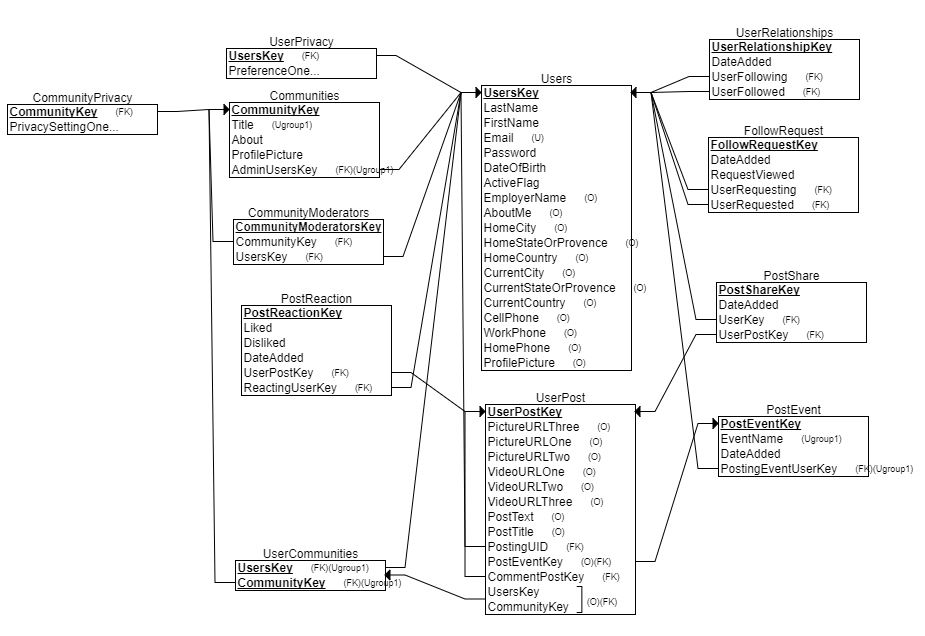
\includegraphics[width=\linewidth]{database.JPG}
  \caption{Current database relational schema.}
\end{figure}
\FloatBarrier
\subsubsection{Users} The Users table stores all of the data for a given user. This includes information like the users name, email, address and more. 
\subsubsection{UserPrivacy} UserPrivacy stores all privacy setting values for a specific user. Current privacy settings are yet to be determined, but as development continues these settings will be added.   
\subsubsection{UserRelationships} This table stores the id's of different users who have established a friendship, also known as "following", with each other.
\subsubsection{FollowRequests} FollowRequests keeps track of the users one has requested to follow as well as who has requested to follow that user.
\subsubsection{UserPost} User post contains all of the data for a post the a user makes. This also defines a comment or reply, but the application itself restricts what data is entered in these cases.
\subsubsection{PostReaction} PostReaction keeps track of likes or dislikes a user has made towards a specific post.
\subsubsection{PostShare} PostShare keeps track of who has shared what post.
\subsubsection{PostEvent} PostEvent stores data that defines an event and allows a user to categorize different posts as an event.
\subsubsection{Communities} Communities stores the data for a specific community as well as who created it, similar in this regard to the Users table. 
\subsubsection{CommunityPrivacy} Similar to userPrivacy, this table stores the data for the settings that a Community has set for it, like is the community publicly viewable or private to added members.
\subsubsection{CommunityModerators}The communityModerators table keeps track of users who have been given moderator privileges for a given Community. 
\subsubsection{UserCommunities} Finally, UserCommunities, keeps track of all of the different communities that users are members of. This was given an intermediary table due to the fact that users can be a member of multiple community pages. 
\subsubsection{Current Database conclusion} So far, all of the user related tables have been written and implemented on PHPmyAdmin. The UI has been connected for the login and sign-up pages, and we're currently working on testing. 
\subsection{Next Steps}
What's next for the database: writing out and implementing the post and posting related tables as well as testing. The final tables are in the works of being written, however, in the meantime testing for correctness for user login and user sign up is being done. Beyond this, we're also testing to ensure sensitive data is being stored correctly and safely. As we progress with the UI development, more and more testing for the database will be done to ensure that data is stored correctly, as well as securely. Discussing the current structure for posting in some more detail, we represent all posts, including comments and replies, as a post. The purpose of this structure is to reduce the number of tables and allow for a more efficient structure. Comments and replies will be implemented this way by restricting what is used application side, so that only the fields required for these two features are used. Comments can also reference the postReaction table, for likes and dislikes, but will not reference the postEvent table (only actual posts can reference this).

\subsection{Problems and Impediments}
One of the bigger problems on designing the back-end of the Kite application, the database, was figuring out what features or pieces of data were going to be handled database side or application side. For instance, as noted in the database section, we ended up reducing the number of tables in regards to posting because we found that representing comments and replies as posts would simplify the database and achieve the same thing as having dedicated tables for comments and replies. Beyond these types of problems, small issues for features we hadn't thought about came into question. For example, our postReaction table has likes and dislikes. We wanted to have a feature that allowed user to respond to a post in this manner, but we hadn't discussed the specific options we wanted users to have in reacting to a post. These types of problems lead to a decline in progress with the development with the database in an effort to reduce unilateral feature decisions for the project. However, this is not in any way a suggestion that the group as a whole wasn't communicating, rather, it was just a small enough feature that we had not discussed how we were going to handle it. Overall, most of these non-discussed features have been handled up to the current development state of the database.  

\subsection{Additional Information}
Besides finishing up the database, we are also working on persistent login using React Native's AsyncStroage library. This will allow users to login and stay logged in even after closing the application so they will remain logged in when they return. A user can shut this off by simply logging out of the application. We find that this will make for a more enjoyable user experience because a user will not have to log in every time they exit the application. This feature will also speed up application testing because we won't have to log in every time we want to test a new or existing feature. 

\section{Back-End - Sawyer Kokesh}

\subsection{Current Development State}
The current state of the back-end for the kite app is a working connection between the database and the front-end in a few of the pages. The connection between the two is done though fetch calls to PHP scripts.The first page that is connected is the signup page which allows the user to register for the app. With this script we handle that creation of new users, this script has some important security concerns that we take care of. One of these concerns is to make sure that the password is hashed to make sure that the passwords are protected within the database. Another thing that the script does to make the data secure is to give each user a random index on creation. The second page is the login page which allows the user to regain access to the Kite app. This also has the ability to verify the password that is hashed. 

\subsection{Next Steps}
The objectives that still need to be completed for the Back-End connections are numerous. For each of the pages the front end has there will need to be php scripts to populate the page with information that is pertinent to that screen. For the Timeline page which is the page that has a sprawling never ending list of post and events that you can scroll though. The php call to gather the information that will populate this page and allow for the scrolling of the page while seamlessly adding the new events that are returned from our calls to the back-end. This will be a changeling UI and back-end connection to set up, but luckily the way we are going to return timeline is done by the newest to oldest which will be a simple search query to do against the database. For the profiles page the page will open with the current users personal information and setting, the important part of this page is to get the query result from the back-end before the user views the page so there isn't a static page that randomly fills up with a bunch of information. But the query for this call will also be simple because it will just return a whole row in the database that relates to the current user. For a single post there is a lot of information to gather before the post can be done. Important things that we will need to make sure to ensure is that our queries are not allowing for any SQL injection into the database, thereby potentially ruining our data or compromising it. But this goes for any time that we are getting input from the user. The next front end page that we will connect to the back end is events. Events are technically set up in the database exactly like post except that the post is connected with other posts. Thereby making this post an event. Finally we have the community page which will have a group of posters that will all possibly have access to post for the community. So when viewing a community we will first have to check permissions. In different cases the viewable information of the screen will be either turned on or off. With each of these calls there we will also need to have checks for each of the values to make sure that the values that were enter are formatted correctly and are of the correct type. 

\subsection{Problems and Impediments}
The main problem with setting up the back-end to begin with was first creating a way to test the php scripts that were being ran. To do this the creation of both a mock react-native app and database were first created, these became a bigger roadblock than first expected because of the fact that react native was still very new for us as well as not have written SQL in quite some time. But once the temp login, signup app was functional by sending and receiving data from the database, the merging of the fetch calls with the current kite application was quite simple. The changing over from using the mock database to the kite database took a bit more time than expected. The problem we had here was the lack of usability when it came to the errors that were given by PHP. Another impediment that we have come across while writing kite is when we hit a roadblock it is hard to get help from our other group members this is because we all picked one part of the project to get familiar with and become main developer of that one section. Lucky, since time has gone on there has been more communication and pair programming which has help us move more quickly though development. One of the first UI problems that we came across what how to hook up all the different forms of navigation for the app. Since navigation is crucial to any app there was a lot of time put into coming up with a streamline way to house the different forms of navigation. Furthermore since react native is still somewhat new the installation of libraries sometime conflict with the current state of the project thereby adding a bit of a headache to a somewhat simple task. In all, the main impediment that the whole group has faced is getting familiar with the languages and tools that we are using. This is from using PHP for back-end calls, JavaScript for react-native, and SQL to write query against the database, as well as constructing the database.  

\subsection {Additional Information}
The one good thing that i like very much about PHP is that they are scripts are very module in a way. For instance as long as they are sent the relevant information they will return the appropriate JSON string. This is quite handy because in the future if a web version of this app is created we just use calls that are web based and not fetch to get the same information. Thereby not having to implement a large section of the project again.


\section{Conclusion}
Moving forward, Kite will begin closing up some parts of the project and begin working of new parts. As the database moves towards the finals steps of completing the database, the main functions of the application such as the Timeline and Events will be given much more attention.

The User Interface has completed its first iteration and navigation is in place so finally the full functionality of the application will begin to take shape. The navigation bars and screens will begin to fill with different pages, timelines, and settings. In addition, to adding all of the parts of the application, it will be essential to quickly work together to bring together the database and the UI so that what is being stored can be used and displayed among the pages of Kite.

Currently only a few tables within the database are left to be written, of which are all in progress. There are a few elements, such as the privacy settings for both users and communities, which will be edited as testing is done when new privacy features are added. Testing what has been implemented is in progress and is one of our main priorities. We are also trying to implement a persistent login system for an improved user experience and for faster testing.

Finally all the parts of the back-end for Kite are moving along quite nicely. We have made good progress when it comes to signing up and logging in. The frameworks for every other PHP script are going to be quite similar to the already laid out scripts. The creation of the new scripts for posts and profiles will be the main attention and will be the brunt of the communication between the front-end and database. 

The Kite application is moving forward at a decent rate and work is being completed in a timely fashion. The next month or so will be essential as the main functionality of the application will be developed and combined with the rest of the components being developed by the Kite team.  

\section{Project Images}
\FloatBarrier
\begin{figure}[h]
\begin{subfigure}{0.5\textwidth}
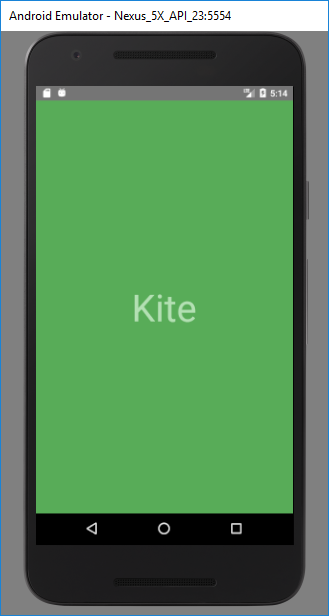
\includegraphics[height=10cm]{Splash.PNG}
  \caption{Current Splash Screen}	
\end{subfigure}
\begin{subfigure}{0.5\textwidth}
  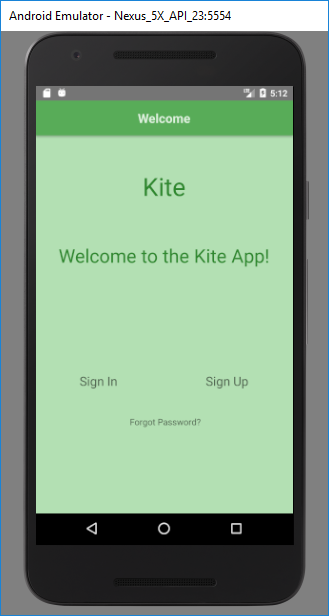
\includegraphics[height=10cm]{welcome.PNG}
  \caption{Current Welcome Screen}
\end{subfigure}
\end{figure}

\begin{figure}[h]
\begin{subfigure}{0.5\textwidth}
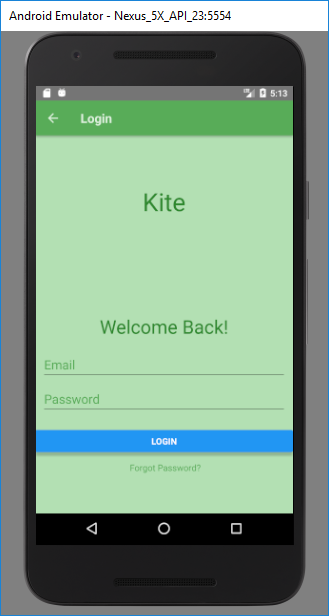
\includegraphics[height=10cm]{login.PNG}
  \caption{Current Login Screen}	
\end{subfigure}
\begin{subfigure}{0.5\textwidth}
  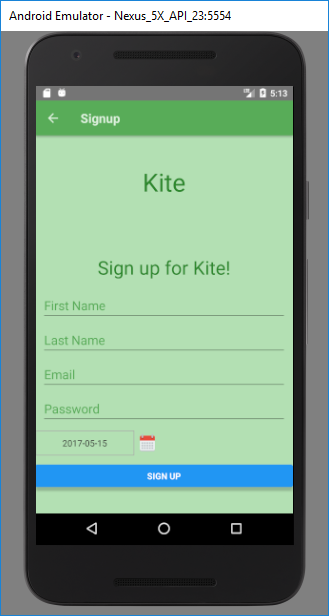
\includegraphics[height=10cm]{Signup.PNG}
  \caption{Current Signup Screen}
\end{subfigure}
\end{figure}
\FloatBarrier

\begin{figure}[h]
\begin{subfigure}{0.5\textwidth}
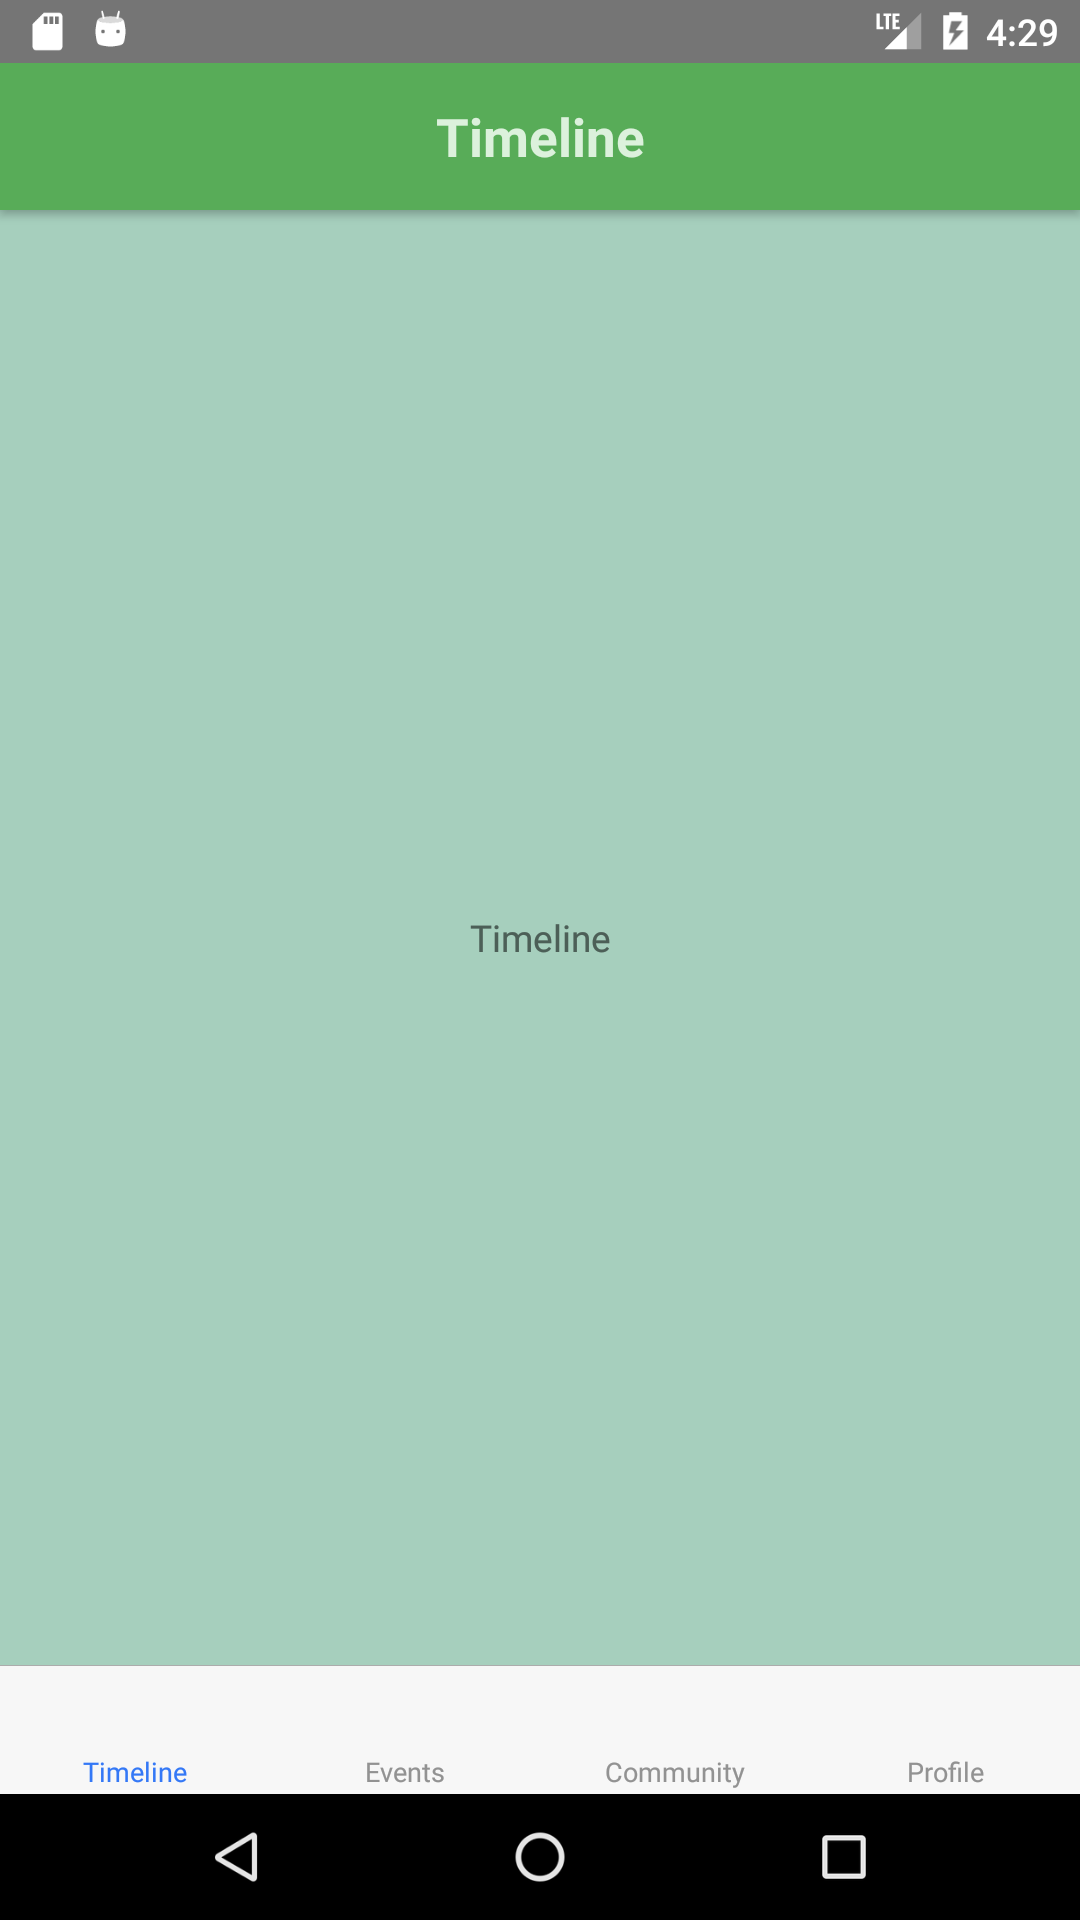
\includegraphics[height=10cm]{timeline.png}
  \caption{Current Timeline Screen}	
\end{subfigure}
\begin{subfigure}{0.5\textwidth}
  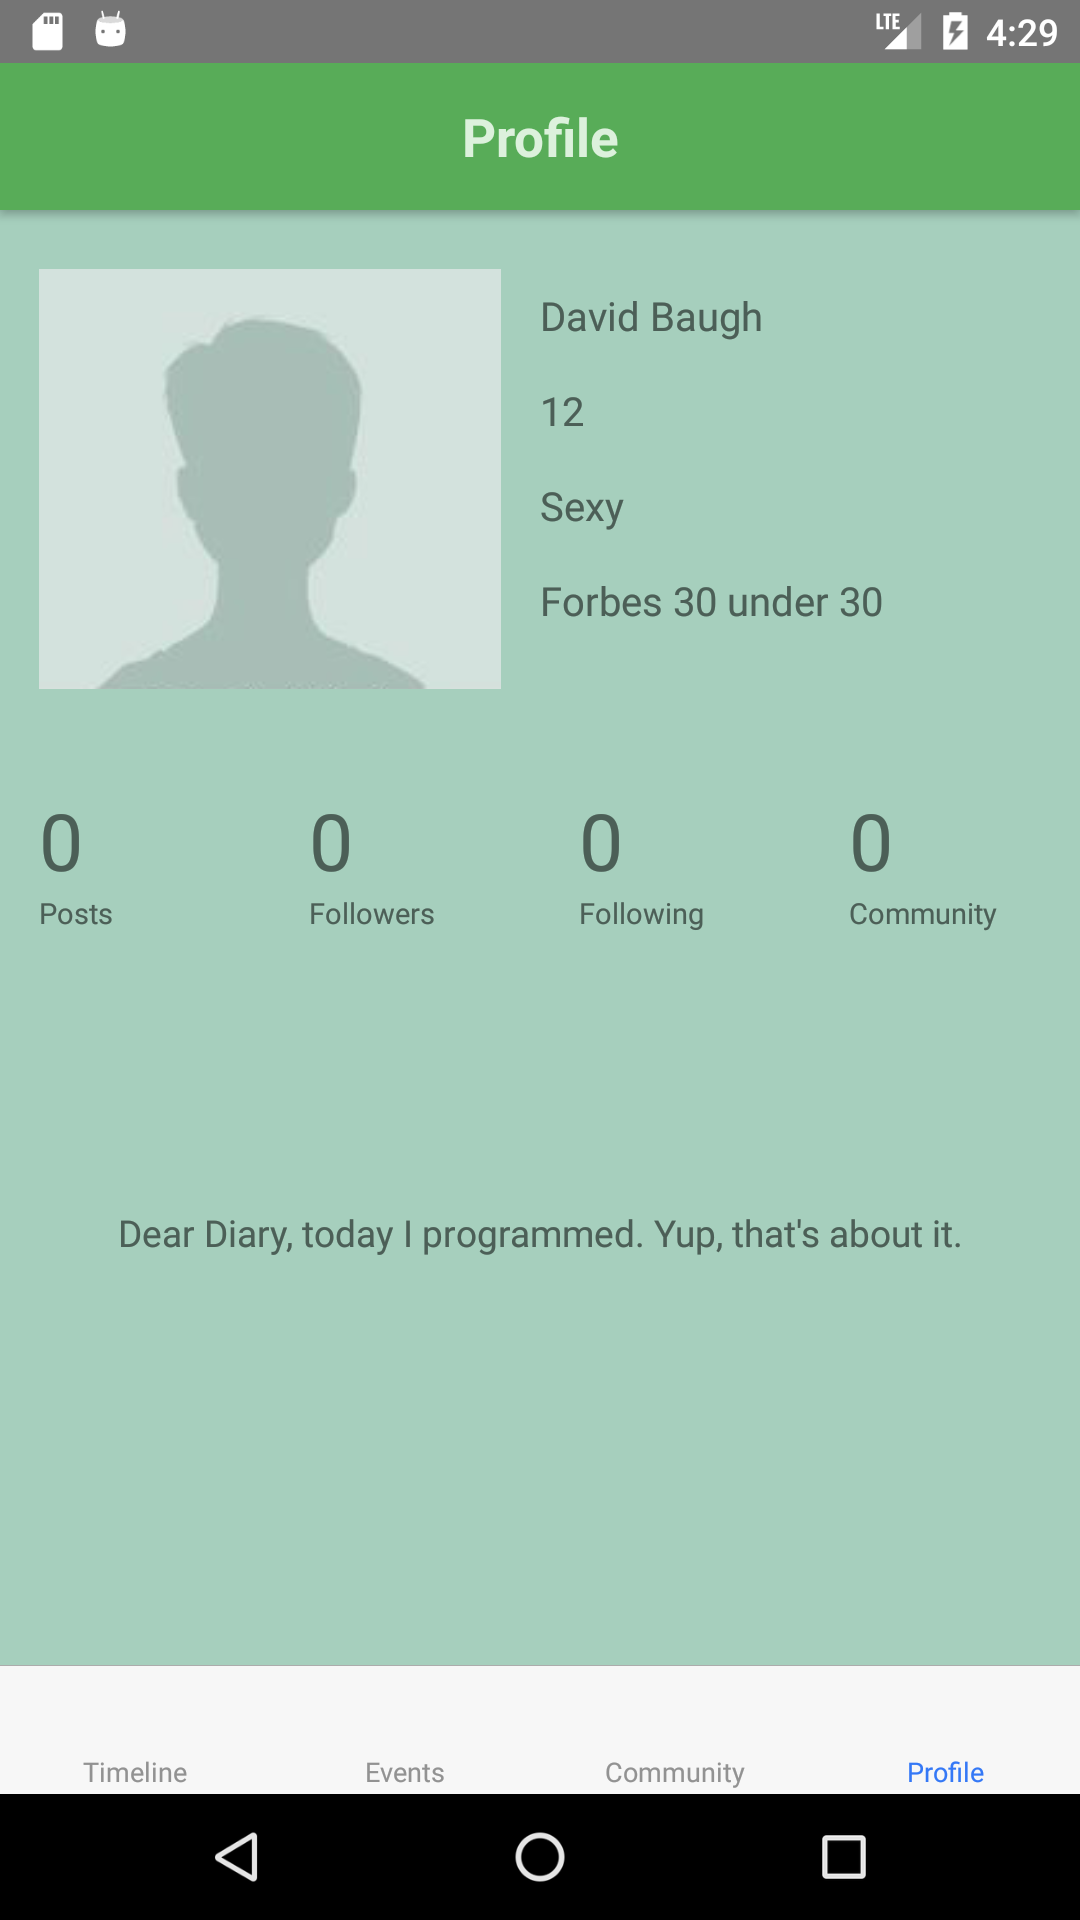
\includegraphics[height=10cm]{profile.png}
  \caption{Current Profile Screen}
\end{subfigure}
\end{figure}
\FloatBarrier

\begin{figure}[h]
\begin{subfigure}{0.5\textwidth}
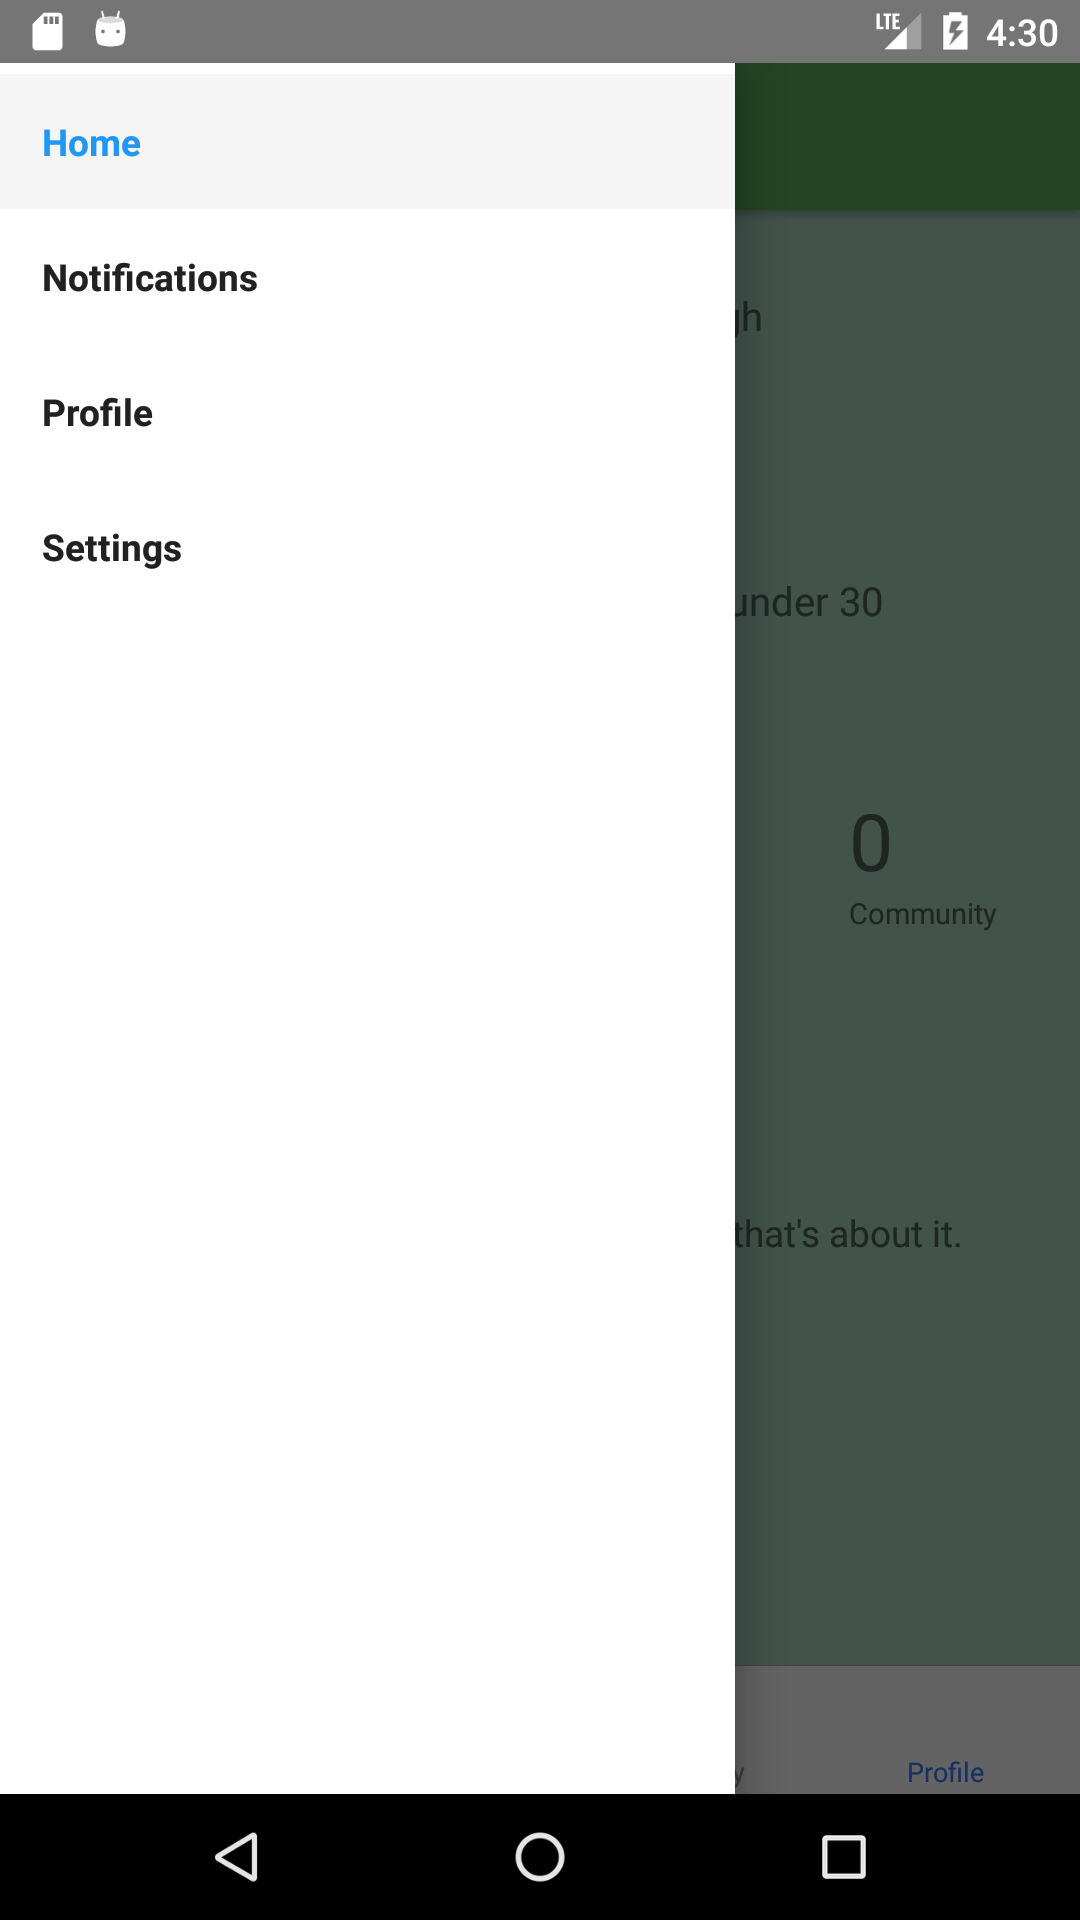
\includegraphics[height=10cm]{drawer.png}
  \caption{Current Drawer Navigation}	
\end{subfigure}
\end{figure}
\FloatBarrier

\end{document}
